\subsection{Principal Component Cosine Analysis}
\label{subsec:pca-cosine}

Principal Component Analysis (PCA) is a dimensionality reduction technique that extracts the most significant information from a dataset while minimizing noise. It achieves this by transforming the data into principal components using the eigenvalues and eigenvectors of the covariance matrix. The components with the highest variance are selected to efficiently represent the dataset \cite{pearsonLIIILinesPlanes1901, jolliffePrincipalComponentAnalysis2002}.

In practice, PCA converts an \(n \times n\) distance matrix into an \(n \times k\) matrix (\(k < n\)). After this transformation, pairwise distances in the reduced space are computed using the cosine distance. The cosine distance between two row vectors \(\mathbf{v_1}\) and \(\mathbf{v_2}\) is defined by:

\begin{equation}
    d_{\cos}(\mathbf{v_1}, \mathbf{v_2}) = 1 - \frac{\mathbf{v_1} \cdot \mathbf{v_2}}{\|\mathbf{v_1}\| \|\mathbf{v_2}\|},
    \label{eq:cosine-distance}
\end{equation}

This method calculates the cosine distances between all pairs \((v_i, v_j)\) for \(i, j \in \{1, 2, \ldots, n\}\), reconstructing a symmetric distance matrix. By using cosine distance, we emphasize directional similarity, which effectively handles high-dimensional data. This provides a computationally efficient approach to reconstruct the distance matrix, allowing us to discern and analyze the underlying structure in the data, isolating the most influential characteristics that define data relationships.

\begin{figure}
    \begin{subfigure}[b]{0.48\textwidth}
        \centering
        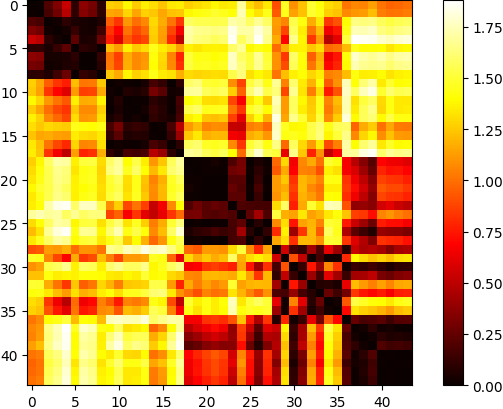
\includegraphics[width=\textwidth]{figures/motion-capture-data/heatmaps/pca_10.png}
        \caption{}
    \end{subfigure}
    \hfill
    \begin{subfigure}[b]{0.48\textwidth}
        \centering
        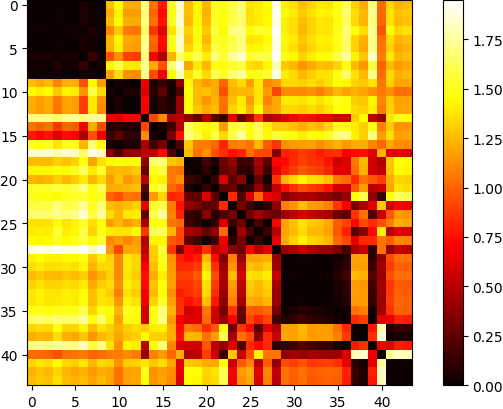
\includegraphics[width=\textwidth]{figures/motion-capture-data/heatmaps/pca_3.png}
        \caption{}
    \end{subfigure}
    \caption[Heat Maps of Cosine Distances after PCA on Reparameterization and Logarithmic Signature Data]{(a) Reparameterization through dynamic programming at a search depth of 10, (b) Logarithmic signature at a truncation level of 3. This figure displays heat maps of the cosine distance matrix following PCA, using data from reparameterization and logarithmic signature as seen in Figure \ref{fig:heatmaps-dynprog} (search depth of 10) and Figure \ref{fig:heatmaps-logsig} (truncation level of 3).}
    \label{fig:heatmap-pca-cosine}
\end{figure}

As shown in both subfigures, the cosine distance matrix after PCA captures the motions as distinct clusters. This indicates that the PCA method effectively reduces the dimensionality of the data, emphasizing the most significant features that define the motion capture data. This also reflects the categorization of the motions, demonstrating PCA's ability to highlight the underlying structure in the data.